\documentclass[11pt,a4paper]{article}
\usepackage[margin=23mm]{geometry}
\usepackage[T1]{fontenc}
\usepackage{lmodern,graphicx,hyperref,fancyvrb,enumitem,tabularx}
\hypersetup{colorlinks=true,urlcolor=blue,linkcolor=blue}
\setlength{\parindent}{0pt}\setlength{\parskip}{7pt}
\setlength{\emergencystretch}{4em}
\setlist[enumerate]{leftmargin=*,itemsep=5pt}
\title{Blender Optical Experiments\\\large From a fresh download to your first figure}
\author{B. M. Rodriguez-Lara \and J. Escamilla Angeles}
\date{5 November 2026}
\begin{document}\maketitle
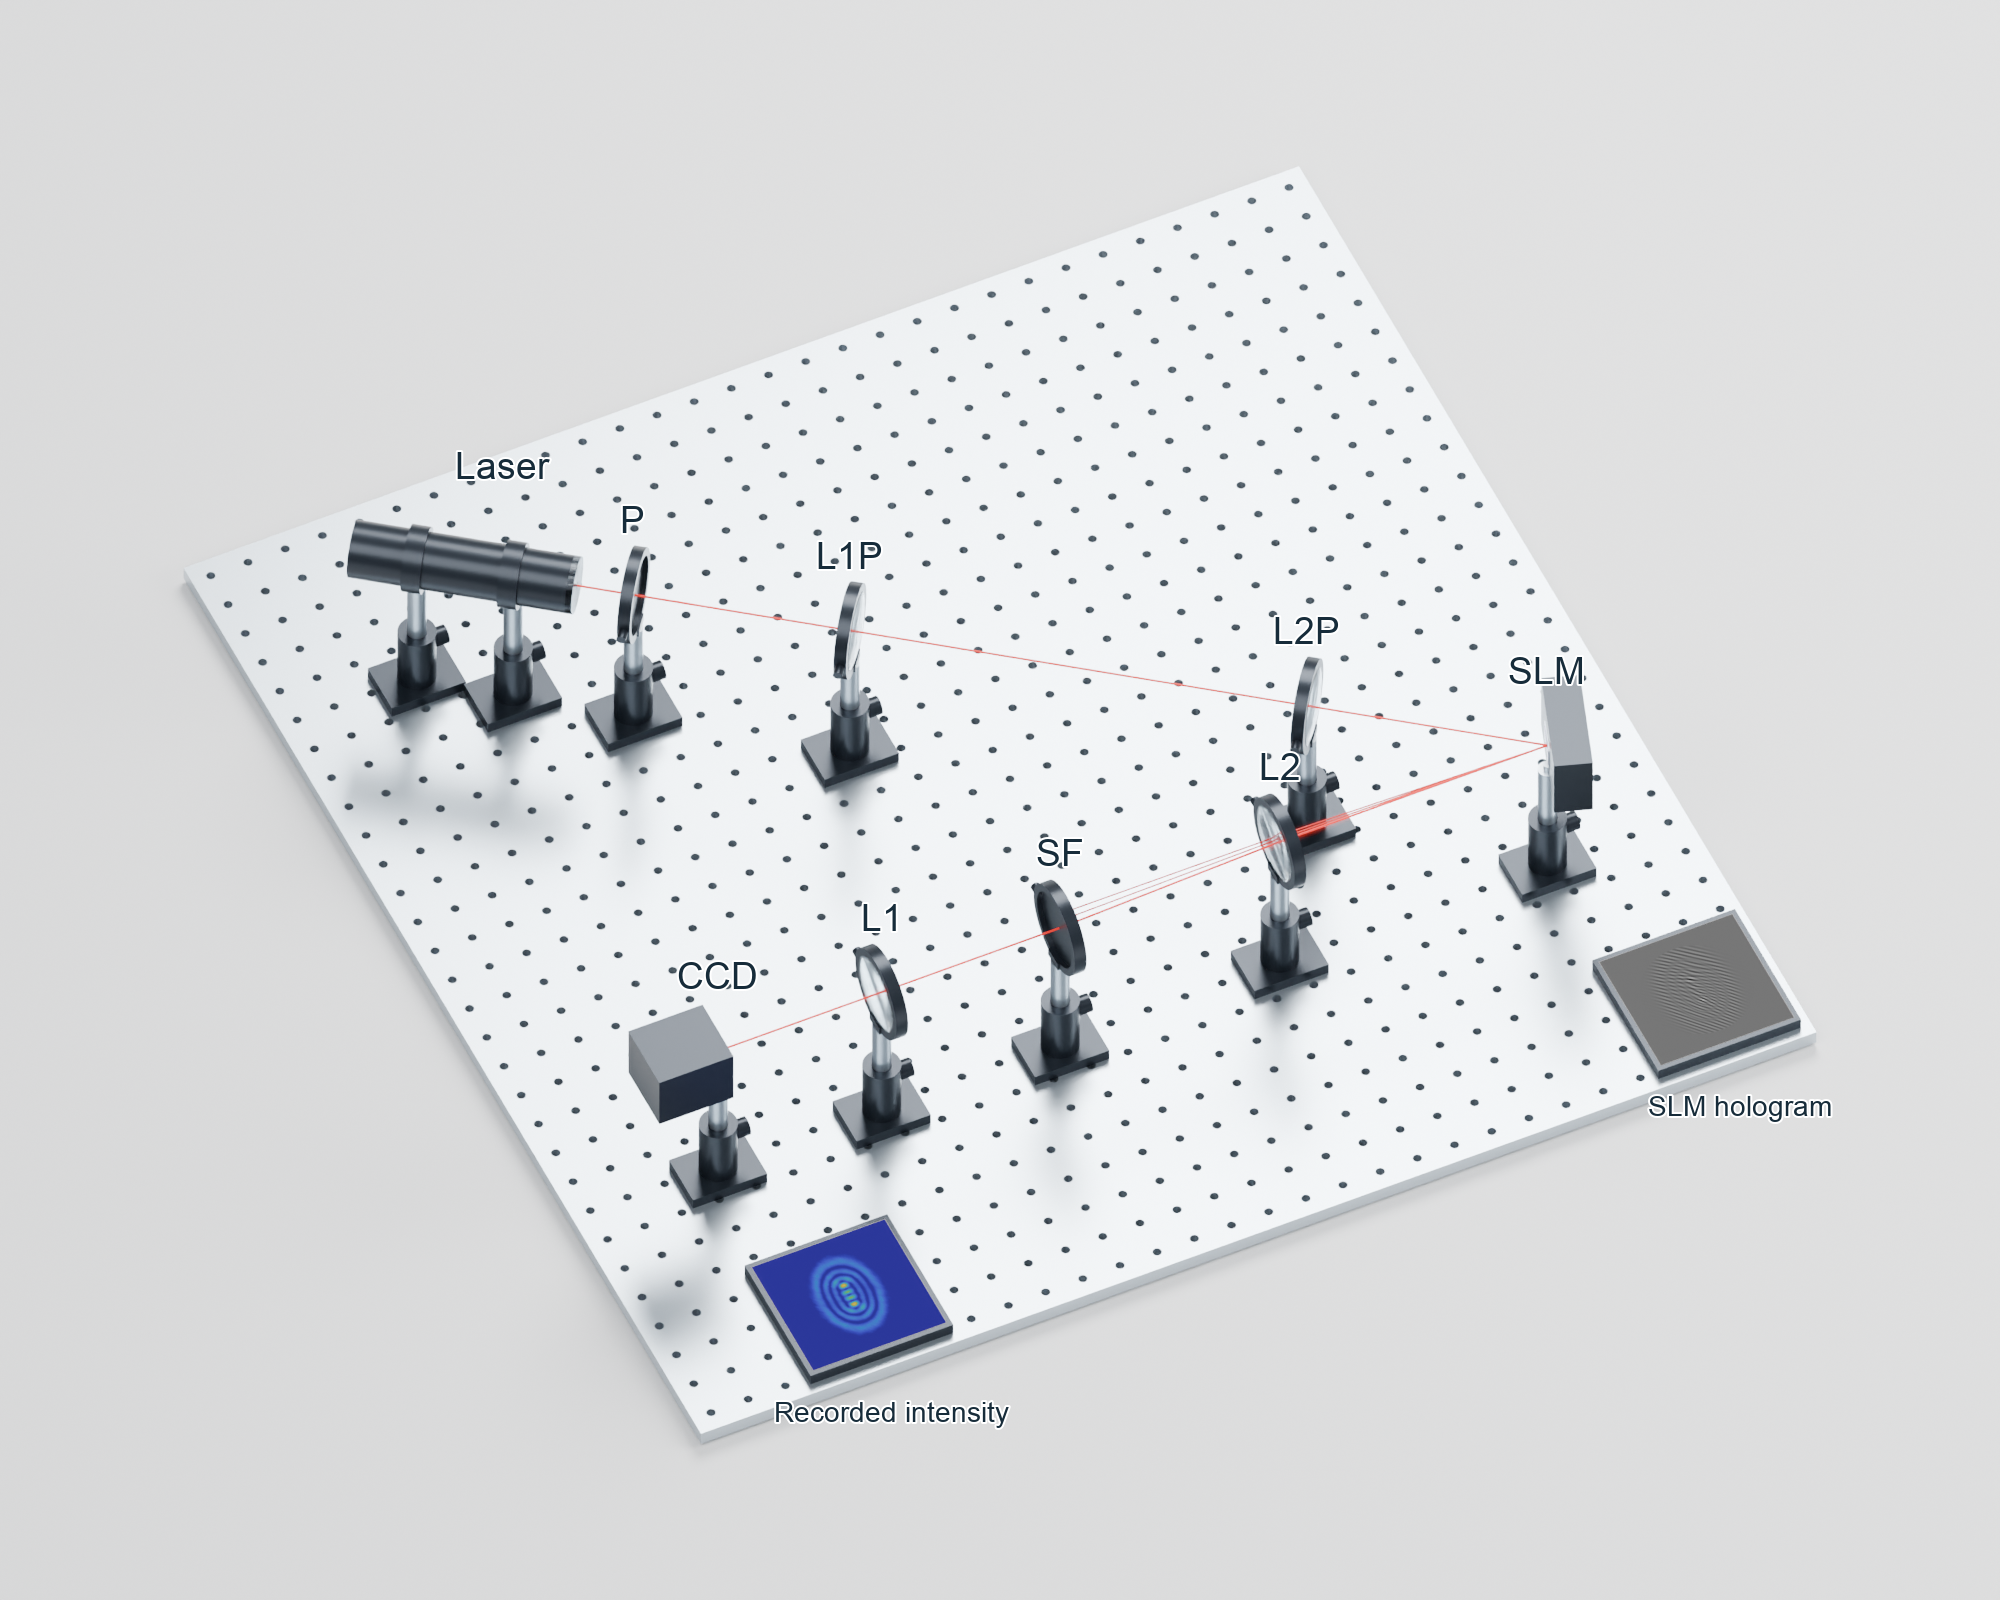
\includegraphics[width=\linewidth,height=.46\textheight,keepaspectratio]{../images/paper-example.png}\par
\medskip
\textbf{What you will make}\par
An optical-bench illustration with a laser, a pupil, four lenses, a reflective spatial light modulator, a spatial filter and a camera. The components sit on generic mounts above a perforated breadboard. Two image panels show the supplied SLM hologram and recorded camera intensity beside their instruments, along the front edge of the table.

This guide takes you from downloading the library to generating this example. It includes the full request to copy into Codex; you do not need to find or assemble instructions from other prompt files.

The basic 2D schematic in \url{https://doi.org/10.1103/6ftp-svh8} inspired this later reconstruction. The paper did not include or use these Blender models. The result is a visualization, not an optical simulation or a fabrication drawing.
\clearpage
\section*{1. Put the project and agent in place}
\begin{enumerate}
\item Install Blender from \url{https://www.blender.org/download/} and launch it once. This example was tested with Blender 5.2.3 LTS. You also need Codex running locally with access to the project folder and permission to run Blender.
\item Open \url{https://github.com/bmlara-github/blender-optical-experiments}. Click \textbf{Code}, then \textbf{Download ZIP}. Extract the ZIP.
\item Move the extracted folder to a location you will keep, such as \path{Documents/OpticalElements/blender-optical-experiments/}. A downloaded folder may end in \texttt{-main}; you may rename it.
\item Keep the following folders together. The folder containing them is the \textbf{project folder}.
\end{enumerate}
\begin{Verbatim}[fontsize=\small]
blender-optical-experiments/
  library/
    Generic_Experimental_Optics.blend
  agent/
    setup-to-blender/
      SKILL.md
  examples/paper-setup/
    layout.json
    reference-images/
      slm_hologram.png
      ccd_intensity.png
  scripts/
  images/
  docs/
\end{Verbatim}
\textbf{Where does the library go?} Leave the \texttt{library/} folder here. Do not move it into the Blender application.

\textbf{Where does the agent go?} Leave the \texttt{agent/} folder beside \texttt{library/}. The agent is a set of instructions for Codex, not a Blender add-on. The direct call in this guide needs no separate agent installation and no hidden folders.

\textbf{Open the project in Codex.} Select this project folder and start a local chat. Choose the folder containing \texttt{README.md}, \texttt{library/} and \texttt{agent/}, not one of those subfolders. Keep this chat open for Step 3.

\textbf{To browse the assets manually in Blender:} open Preferences, find Asset Libraries (under File Paths in some versions), click Add and select this project's \texttt{library/} folder. Name it ``Optical Experiments.'' Change an editor area to Asset Browser and select that library. This browsing setup is optional for the scripted example, which loads the library directly.
\clearpage
\section*{2. Understand the example before generating it}
Follow the light from the laser to the camera:
\begin{center}
\textbf{Laser $\rightarrow$ P $\rightarrow$ L1P $\rightarrow$ L2P $\rightarrow$ SLM}\\[5pt]
\textbf{SLM $\rightarrow$ L2 $\rightarrow$ SF $\rightarrow$ L1 $\rightarrow$ CCD}
\end{center}
The path changes direction at the reflective SLM. The second line above continues the same path; it does not introduce a second SLM.

\renewcommand{\arraystretch}{1.25}
\begin{tabularx}{\linewidth}{@{}p{20mm}X@{}}
\textbf{Label} & \textbf{Meaning in this example}\\\hline
Laser & Source of the incident beam.\\
P & Circular pupil that limits the incident beam aperture. It is not a polarizer.\\
L1P, L2P & Two lenses on the incident path before the SLM. The illustration shows the beam narrowing and widening through this part of the setup; this is an authored envelope, not a calculated propagation result.\\
SLM & Reflective spatial light modulator displaying the supplied hologram. The outgoing path contains the illustrated $+1$, $0$ and $-1$ diffraction orders.\\
L2 & First lens after reflection at the SLM, before the spatial filter.\\
SF & Spatial filter. Its opening passes the selected $+1$ order; the $0$ and $-1$ orders stop at the filter.\\
L1 & Lens between the filter and the camera. Only the selected order continues along this path.\\
CCD & Camera recording the output intensity. Its nearby panel shows the supplied intensity image.\\
\end{tabularx}

\textbf{How the scene is arranged.} A 750 by 750 mm breadboard supports the optics on posts, holders and mounts. The optical axis is 120 mm above its top. The SLM and CCD panels lie flat at matching height along the front edge, each near its associated instrument. There are no table legs or panel connector lines.

\textbf{What the dimensions mean.} The board size, positions, mounting choices, 4 mm pupil and 1 mm filter opening are visualization assumptions. They are not measurements of the published apparatus. Focal lengths are unspecified; the library uses generic biconvex lenses. Do not infer a magnification or a calibrated relay from the drawing.

\textbf{Labels and images.} This reconstruction retains L2 nearest the SLM and L1 nearest the CCD. Earlier source notes reported inconsistent lens naming between the drawing and manuscript prose; these are the labels used here. The two image panels are supplied reference images, not simulated results. The full paper drawing is not bundled.
\clearpage
\section*{3. Copy this complete request into Codex}
Paste the entire block below into the project chat opened in Step 1. It contains the system description and the requested outputs. No separate prompt file needs to be opened. The agent uses the bundled layout only for coordinates and orientations.
\begin{Verbatim}[fontsize=\small,baselinestretch=0.94]
Read agent/setup-to-blender/SKILL.md and generate this figure.

Create a realistic-looking optical experiment on a generic
750 x 750 mm perforated breadboard, without table legs.
Use this project's generic library and collection instances
at unit scale (1 Blender unit = 1 meter). Set the optical
axis 120 mm above the tabletop. Use posts, holders and lens
mounts to support the components.

The beam follows this sequence:
Laser -> P -> L1P -> L2P -> SLM -> L2 -> SF -> L1 -> CCD.

P is a circular pupil, not a polarizer. L1P and L2P are the
two lenses before the reflective spatial light modulator
(SLM). At the SLM, fold the path toward L2, SF, L1 and CCD.
L2 is the lens nearest the SLM; L1 is nearest the CCD.
SF is a spatial filter: transmit the +1 diffraction order
toward L1 and CCD; stop the 0 and -1 orders at SF.
Do not add a beam splitter or a polarizer.

Use generic biconvex lenses. Focal lengths are unspecified;
do not invent them. For this illustration use a 4 mm pupil
and a 1 mm filter opening. Use examples/paper-setup/layout.json
for coordinates and orientations, not as measured data.
Draw continuous red beams. Make rejected orders dimmer in
the same red hue. Do not add direction arrows.

Include the two images in
examples/paper-setup/reference-images/:
- slm_hologram.png: a flat framed panel beside the SLM.
- ccd_intensity.png: a flat framed panel beside the CCD.
Put both panels along the front table edge, at the same
height and with their centers at Y = -0.25 m. Preserve
aspect ratios and pack the images in the Blender file.
Do not draw connector lines or invent replacement images.

Use scripts/build_generic_example.py for this example and
scripts/export_example.py for the SVGs. Locate Blender and
check the exporter's Pillow dependency before running.
Save in a new Figures/YYYY-MM-DD-FIgNN/ folder using my
local date and the next unused number. Preserve prior files.

Render perspective and overhead views at 2000 x 1600 pixels,
40 Cycles samples, with denoising. Deliver the editable
Blender scene, repeatable source, clean and lettered PNGs,
and paired SVGs with/without editable text at 86 mm width.
Keep the optical render raster and the SVG text editable.
Inspect both views. Report missing files or failures, and
record assumptions and checks in the figure README.
Generate the files now and give me links to the outputs.
\end{Verbatim}
\clearpage
\section*{4. Open and check your results}
When rendering finishes, Codex should provide links to a new figure folder. For example, the first figure on 5 November 2026 would use \path{Figures/2026-11-05-FIg01/}; later figures use the next unused number.
\begin{Verbatim}[fontsize=\small]
Figures/YYYY-MM-DD-FIgNN/
  example.blend             Editable scene, with packed images
  build_source.py           Repeatable Blender source
  setup.json                Scene description and assumptions
  instances.json            Components and placements
  validation.json           Recorded checks
  README.md                 Notes and limitations
  source/                   Copies of the two image panels
  renders/
    example-perspective-clean.png
    example-perspective-lettered.png
    example-plan-clean.png
    example-plan-lettered.png
  svg/
    example-perspective-lettered-86mm.svg
    example-perspective-unlettered-86mm.svg
    example-plan-lettered-86mm.svg
    example-plan-unlettered-86mm.svg
\end{Verbatim}
\begin{enumerate}
\item Open \texttt{example.blend} in Blender to move components, change materials or adjust the cameras. Save edited variants under a new name.
\item Open both rendered views. Follow the beam through P, L1P, L2P, SLM, L2, SF, L1 and CCD. Confirm that rejected orders stop at SF and both image panels are visible at the front edge.
\item Use the clean PNG for an unlabelled image, or the lettered PNG for an immediate preview with labels.
\item Open a lettered SVG in your vector editor to edit the text. Its optics are an embedded raster image; only the lettering is vector. The default width is 86 mm, with the image aspect ratio preserved.
\item Read the README and checks before using the figure. Recorded geometry checks do not establish optical performance or mechanical compatibility.
\end{enumerate}
\textbf{If Blender is missing:} give Codex its executable path. On macOS this is commonly \path{/Applications/Blender.app/Contents/MacOS/Blender}. On Windows, locate \texttt{blender.exe} in the installed Blender folder.

\textbf{If Pillow is missing:} ask Codex to install it in a project-local Python environment and rerun the exporter. Blender's renderer and the PNG/SVG exporter use separate Python environments.

\textbf{If only a plan appears:} ask Codex to run the supplied builder and exporter and inspect the resulting files. A completed result includes both rendered views, not just a script or a default Blender cube.
\clearpage
\section*{5. Describe your own experiment}
Keep the library and agent in their existing folders. Put your sketch and image panels inside a new \texttt{inputs/} subfolder, for example \path{inputs/my-experiment/}. A hand-drawn sketch is useful if it shows the optical order, folds and branches. Label its components consistently with your list.

For a custom setup, provide these details directly in your request:
\begin{itemize}[leftmargin=*]
\item Components, in the order encountered by the beam, including every branch or repeated pass.
\item What each label means, which lenses have known focal lengths, and any known apertures or distances with units. Say ``unknown'' when a value is unavailable.
\item Mounting style, table size and optical height, or permission to choose illustrative dimensions.
\item The filename of your sketch, and the filename and associated instrument for each image panel.
\item The views, publication width and labels you want in the finished figure.
\end{itemize}
Here is a complete small example you can adapt. The values below are illustrative choices for a different scene, not values from the paper:
\begin{Verbatim}[fontsize=\small]
Read agent/setup-to-blender/SKILL.md. Create a new figure
using this project's generic experimental library.

My setup is Laser -> circular pupil P -> lens L -> CCD.
Use a straight beam path. The focal length of L is unknown.
Use a 450 mm square breadboard, a 120 mm optical height,
and generic mounts. Choose clear illustrative spacings
and record those choices. Use a 4 mm pupil opening.

I have no sketch or detector image for this example.
Do not invent a detector intensity panel.
Generate perspective and overhead views, clean and
lettered PNGs, and paired SVGs at 86 mm width. Label
Laser, P, L and CCD. Save the Blender scene, repeatable
source and notes in a new dated Figures folder.
Adapt a copy of the builder for this new optical path;
do not run the unchanged paper-example layout.
Render, inspect the result and give me the output links.
\end{Verbatim}
To use your own files, add a sentence such as: ``My sketch is \texttt{inputs/my-experiment/sketch.png}. My camera image is \texttt{inputs/my-experiment/ccd.png}; place it beside CCD.'' The agent should interpret those inputs and adapt the scene, not silently reuse the paper setup.

\section*{6. Library, documentation and rights}
The 39 generic assets are reusable collection assets. Keep their source instance scale at $(1,1,1)$: one Blender unit is one meter. Catalogue display sizes are normalized for browsing and are not a common physical scale.

Original code uses MIT; original models and documentation use CC BY 4.0. Supplied reference images retain their existing rights. See LICENSE and \texttt{docs/provenance.md}. Common laboratory optomechanics, including Thorlabs equipment, inspired the generic designs; this project is not affiliated with or endorsed by Thorlabs.


\clearpage
\section*{7. How to cite}
If you use this library in a publication, please cite the project:

Rodriguez-Lara, B. M., and Escamilla Angeles, J. (2026).
\textit{Blender Optical Experiments} [Computer software]. Zenodo.
\url{https://doi.org/10.5281/zenodo.23997720}.

\textbf{Permanent project DOI (all versions):}
\url{https://doi.org/10.5281/zenodo.23997720}

This is Zenodo's ``Cite all versions'' DOI. It remains the project citation as new releases are published and resolves to the latest version. The citation intentionally omits a release number. You may state the version used separately in your methods for reproducibility.

\subsection*{BibTeX for LaTeX}
Copy this entry into your bibliography file, or import
\path{docs/citations/experiments-project.bib}:
\VerbatimInput[fontsize=\small]{citations/experiments-project.bib}
Cite it in your manuscript with:
\begin{Verbatim}[fontsize=\small]
\cite{rodriguez_lara_escamilla_2026_optical_experiments}
\end{Verbatim}
\subsection*{Other formats}
All files are supplied in \path{docs/citations/}:
\begin{itemize}
\item \texttt{experiments-project.ris}: import into a reference manager that supports RIS.
\item \texttt{experiments-project.csl.json}: structured citation metadata for tools that accept CSL-JSON.
\item \texttt{experiments-project.txt}: a plain-text reference to copy into a document.
\end{itemize}
In reference managers that support DOI lookup, you can also paste the permanent DOI above and check that both authors appear in the stated order.

\textbf{The scientific paper is a separate work.} Cite its DOI when discussing its science or setup. The paper's basic 2D schematic motivated this later Blender project; the paper did not include or use these models. The paper citation does not replace the library citation.

The editable guide is \texttt{docs/user-guide.tex}. Run \texttt{pdflatex user-guide.tex} twice from \texttt{docs/} to rebuild the PDF. The catalogue is separate from this guide.
\end{document}
